\chapter{Background}
\label[chapter]{chapter:background}

This chapter summarizes background information that may be useful to better understand the method and implementation that will be outlined in the following two chapters. \Cref{sec:coordinate_systems} defines the different coordinate systems applied in the project, while \Cref{sec:coordinate_transformations} outlines methods for coordinate transformations. \Cref{sec:camera_model} describes the camera model used for reprojection and undistortion, and \Cref{sec:iterative_closest_point_algorithm} summarizes the Iterative Closest Points (ICP) algorithm.

\section{Coordinate Systems}
\label{sec:coordinate_systems}

Three different coordinate systems are used for the purpose of this project: world,  GPS, and camera frame. The world frame is constant and given in UTM coordinates, used by the map information. The GPS frame is the time-variant position of the GPS sensor, while the camera frame is the time-variant position of the camera on the train.

\begin{figure}[h]
\begin{center}
    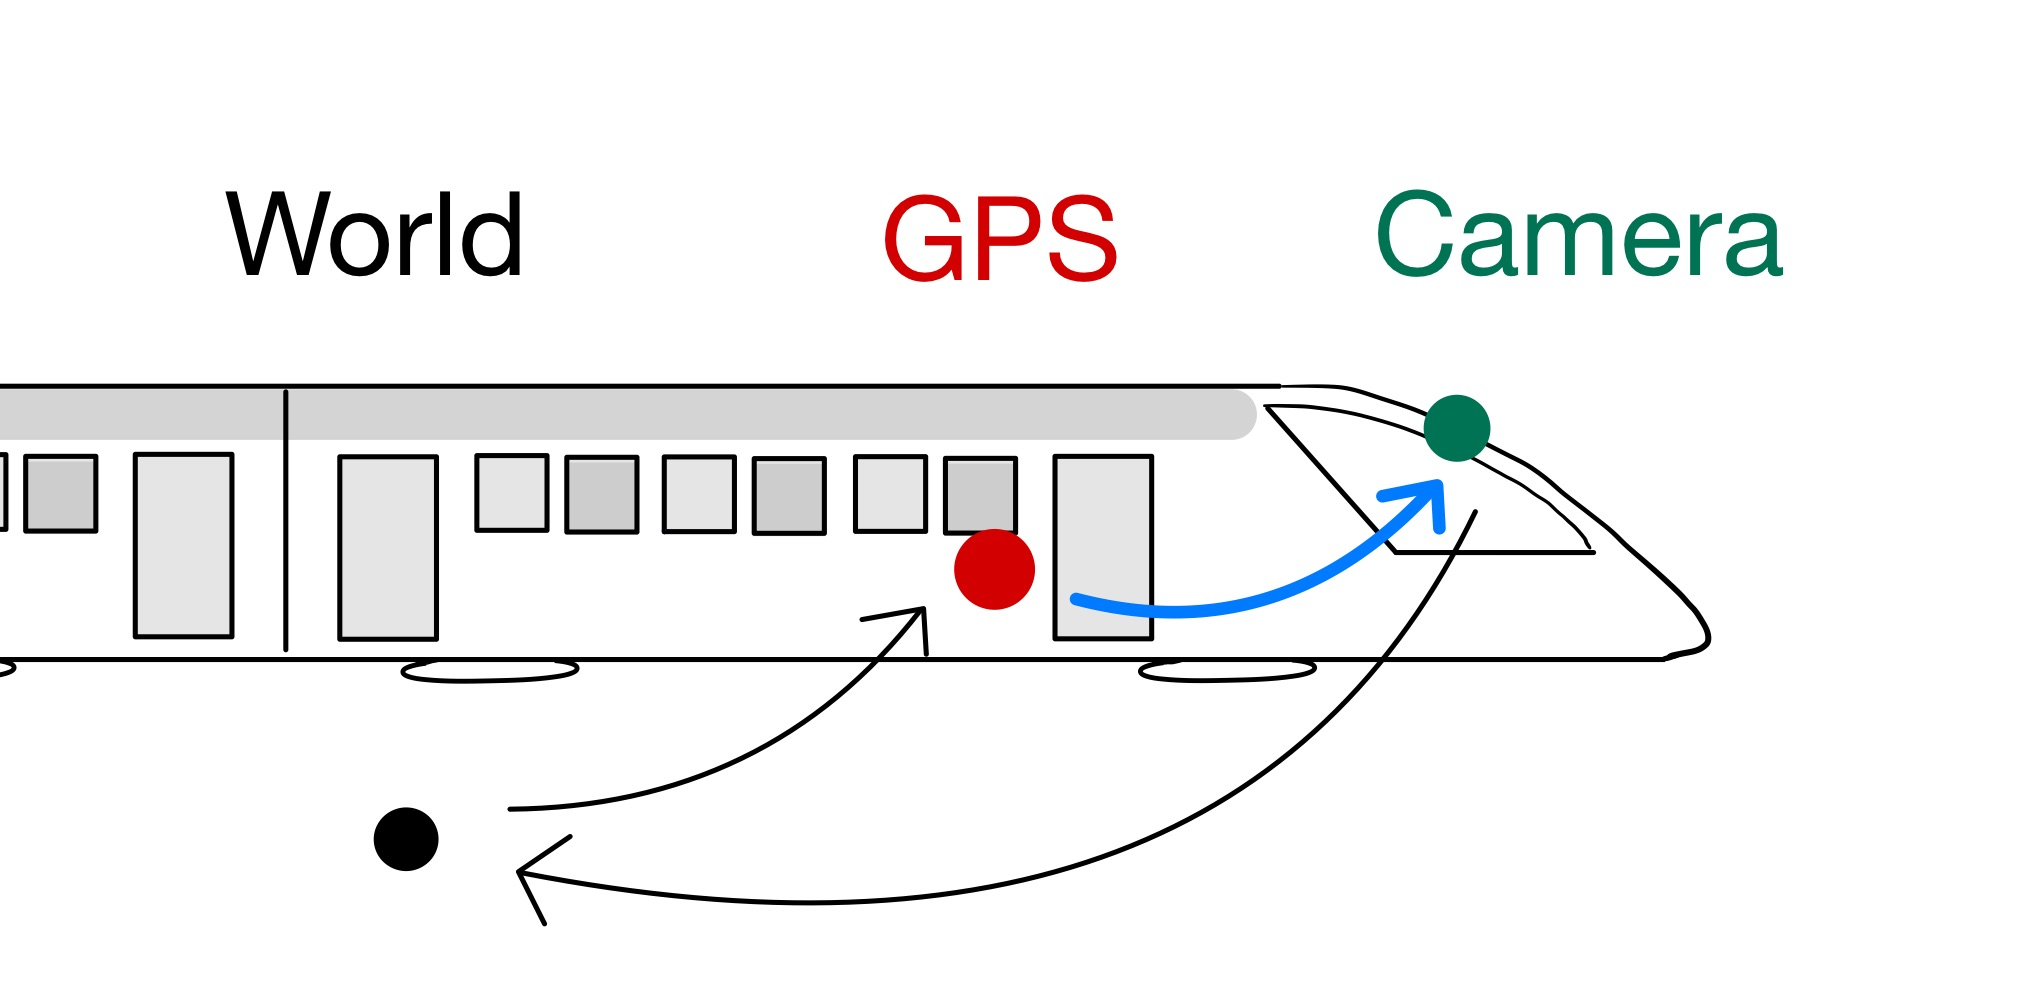
\includegraphics[width=0.5\textwidth]{images/coordinate_systems}
    \caption{World, GPS, and camera coordinate systems illustrated, with the arrows implying their relative transformations \cite{spiegelhalter2023extrinsics}.}
    \label[figure]{fig:coordinate_systems}
\end{center}
\end{figure}

\Cref{tab:axis_directions} provides a comparison of the axis directions in the GPS and camera frames. In the GPS frame the X-axis points forward, the Y-axis to the right of the train, and the Z-axis upwards, whereas in the camera frame the Z-axis points forward, the X-axis to the right of the train, and the Y-axis downwards. The camera frame is defined such that the camera points in the direction of the Z-axis, and the width and height of the image are along the X- and Y- axes, respectively.

\renewcommand{\arraystretch}{1.2}

\begin{table}[h]
    \centering
    \caption{Definitions of directions and associated rotations, in terms of GPS and camera coordinate systems.}
    \begin{tabular}{ l l l l }
        \toprule
        \textbf{Direction} & \textbf{Rotation} & \textbf{GPS Frame} & \textbf{Camera Frame} \\ 
        \midrule
        Longitudinal (forward)      & Roll  & $+X$ & $+Z$ \\ 
        Lateral (sideways, right)   & Pitch & $+Y$ & $+X$ \\ 
        Vertical (upwards)          & Yaw   & $+Z$ & $-Y$ \\
        \bottomrule
    \end{tabular}
    \label[table]{tab:axis_directions}
\end{table}


\section{Coordinate Transformations}
\label{sec:coordinate_transformations}

In order to efficiently transform points between different coordinate systems, two different representations have been used for this project. Firstly, homogeneous transformation matrices are used most of the time since they are more intuitive and simple. Secondly, however, quaternions are used for optimization, where they are dynamically adapted, since they are not prone to numerical singularities.

\subsection{Homogeneous Transformation Matrix}

Transformation, including both translation and rotation, of a vector to point $P$, from initial frame $\mathcal A$ to frame $\mathcal B$. This is achieved using the rotation matrix $R_{\mathcal B \mathcal A}$ (notation: frame $\mathcal A$ to frame $\mathcal B$) and translation vector $_\mathcal B \vec t_{BA}$ (notation: from point $A$ to point $B$, expressed in frame $\mathcal B$). To avoid computation issues, it is crucial to remember which frames the vectors are expressed in.

The homogeneous transformation can be written as a simple Equation (\Cref{eq:homogeneous_transformation}) or combined in the form of a matrix $H_{\mathcal B \mathcal A}$ ()\Cref{eq:homogeneous_transformation_matrix}).

\begin{align}
    _\mathcal B \vec r_{BP} &= _\mathcal B \vec t_{BA} + R_{\mathcal B \mathcal A} \cdot _\mathcal A \vec r_{AP}
    \label[equation]{eq:homogeneous_transformation}
    \\
    \\
    \begin{bmatrix} _\mathcal B \vec r_{BP} \\ 1 \end{bmatrix} &= \underbrace{\begin{bmatrix} R_{\mathcal B \mathcal A} & _\mathcal B \vec t_{BA} \\ \vec 0_{1\times 3} & 1 \end{bmatrix}}_{H_{\mathcal B \mathcal A}} \cdot \begin{bmatrix} _\mathcal A \vec r_{AP} \\ 1 \end{bmatrix}
    \label[equation]{eq:homogeneous_transformation_matrix}
\end{align}

To determine the inverse of a homogeneous transformation matrix, the translation vector need not only be reversed but also rotated to the new frame, while the rotation matrix is simply transposed. This results in the composition as in \Cref{eq:homogeneous_transformation_matrix_inverse}.

\begin{equation}
    H_{\mathcal A \mathcal B} = \begin{bmatrix} R_{\mathcal A \mathcal B} & _\mathcal A \vec t_{AB} \\ \vec 0_{1\times 3} & 1 \end{bmatrix}
    = \begin{bmatrix} R_{\mathcal B \mathcal A}^T & -R_{\mathcal B \mathcal A}^T \cdot _\mathcal B \vec t_{BA} \\ \vec 0_{1\times 3} & 1 \end{bmatrix}
    \label[equation]{eq:homogeneous_transformation_matrix_inverse}
\end{equation}

\newpage
\subsection{Quaternion Rotation}

An effective mathematical tool that can be used to express rotations are quaternions. A quaternion $\vec q$ is a 4D vector with the elements $q_w$, $q_x$, $q_y$, and $q_z$ (\Cref{eq:quaternion_definition}). Its conjugate $\vec q^*$ is the same rotation in the opposite direction.

\begin{equation}
    \vec q = q_w + q_x\cdot \vec i + q_y\cdot \vec j + q_z\cdot \vec k = \begin{bmatrix} q_w \\ q_x \\ q_y \\ q_z \end{bmatrix} \qquad
    \vec q^* = \begin{bmatrix} q_w \\ -q_x \\ -q_y \\ -q_z \end{bmatrix}
    \label[equation]{eq:quaternion_definition}
\end{equation}

In order to rotate a vector $\vec r$ using a quaternion $\vec q$, the quaternion product $\otimes$ is used (equal to the cross-product minus the dot-product), see \Cref{eq:quaternion_rotation}. Note that the quaternion $\vec q$ must be a unit quaternion, i.e. scaled to unit norm.

\begin{equation}
    \begin{bmatrix} 0 \\ _\mathcal B \vec r \end{bmatrix} = \vec q_{\mathcal B \mathcal A} \otimes \begin{bmatrix} 0 \\ _\mathcal A \vec r \end{bmatrix} \otimes \vec q_{\mathcal B \mathcal A}^*
    \label[equation]{eq:quaternion_rotation}
\end{equation}

\section{Camera Model}
\label{sec:camera_model}

This section describes the camera model used in this project. Firstly, the reprojection of 3D points to 2D pixel coordinates is described, followed by the undistortion of the image.

\subsection{Reprojection}
\label{subsec:reprojection}

Following the pinhole camera model \cite{dawson1994simple}, coordinates $(x,y,z)$ in the camera frame are reprojected to pixel coordinates $(u,v)$ in the image plane using \Cref{eq:camera_projection}. The variables $f_x$ and $f_y$ are the focal lengths in pixels, while $c_x$ and $c_y$ are the principal point coordinates in pixels.

\begin{equation}
    u = f_x \cdot \Big(\frac{x}{z}\Big) + c_x
    \qquad
    v = f_y \cdot \Big(\frac{y}{z}\Big) + c_y
    \label[equation]{eq:camera_projection}
\end{equation}

This can also be written in matrix form (\Cref{eq:camera_projection_matrix}), using the camera instrinsics matrix $K$. The variable $\lambda$ is the depth scaling factor, since infinitely many 3D points along a line would project to the same 2D point.

\begin{equation}
    \lambda \begin{bmatrix} u \\ v \\ 1 \end{bmatrix} = \underbrace{\begin{bmatrix} f_x & 0 & c_x\\ 0 & f_y & c_y \\ 0 & 0 & 1 \end{bmatrix}}_K \cdot \begin{bmatrix} x \\ y \\ z \end{bmatrix}
    \label[equation]{eq:camera_projection_matrix}
\end{equation}

\subsection{Undistortion}
\label{subsec:undistortion}

Image distortion means that the camera does not follow the pinhole camera model perfectly. The image is distorted by radial distortion and tangential distortion, as shown in \Cref{fig:radial_tangential_distortion}.

\begin{figure}[h]
    \centering
    \includegraphics[height=0.32\textwidth]{images/distortion_radial.png}
    \hspace{0.1\textwidth}
    \includegraphics[height=0.36\textwidth]{images/distortion_tangential.png}
    \caption{Radial distortion (left) and tangential distortion (right) \cite{weng1992camera}.}
    \label{fig:radial_tangential_distortion}
\end{figure}

Since the initial images are distorted, they first need to be undistorted given the camera intrinsics that include the distortion coefficients. %($k_1$, $k_2$, $k_3$, $k_4$).
The distortion is equidistant and addressed using the OpenCV fisheye model \cite{opencv-fisheye}. %, which uses the following equations for undistortion.

% \Cref{eq:distortion_angle} calculates the angle $\theta$ of the distorted point $(x,y)$, which is then used to calculate the distortion $\theta_d$ using \Cref{eq:distortion_coefficients}. The undistorted point $(x',y')$ is then calculated using \Cref{eq:distortion_points}, and finally the pixel coordinates $(u,v)$ are calculated using \Cref{eq:undistortion_projection_no_matrix}.

% \begin{equation}
%     a = \frac{x}{z} \qquad b = \frac{y}{z} \\
%     r = \sqrt{a^2 + b^2} \\
%     \theta = \arctan(r)
%     \label{eq:distortion_angle}
% \end{equation}

% \begin{equation}
%     \theta_d = \theta (1+ k_1\cdot\theta^2 + k_2\cdot\theta^4 + k_3\cdot\theta^6 + k_4\cdot\theta^8)
%     \label{eq:distortion_coefficients}
% \end{equation}

% \begin{equation}
%     x' = a \cdot \frac{\theta_d}{r} \qquad y' = b \cdot \frac{\theta_d}{r}
%     \label{eq:distortion_points}
% \end{equation}

% \begin{equation}
%     u = f_x \cdot x' + c_x \qquad v = f_y \cdot y' + c_y
%     \label{eq:undistortion_projection_no_matrix}
% \end{equation}

\section{Iterative Closest Point (ICP) Algorithm}
\label{sec:iterative_closest_point_algorithm}

The ICP algorithm \cite{zhang1994iterative} \cite{besl1992method} is an iterative method for aligning two point clouds. It is commonly used in robotics for estimating the pose of a robot with respect to a known map, or for estimating the relative pose between two point clouds.

The algorithm iteratively minimizes the sum of squared distances between the points in the two point clouds. Initialized with an initial guess of the relative pose between the two point clouds, at each iteration, the points in the second point cloud are transformed using the current estimate of the relative pose. The closest points in the first point cloud are then found for each point in the second point cloud. The relative pose is then updated using the closest points. This process is repeated until the relative pose converges.

In the context of this project, the algorithm is used to minimize the 2D residuals between reprojected points and observed image points. The reprojected points are obtained by transforming 3D points using a relative pose estimate, and then reprojecting them onto the image plane using the known camera model. After finding the closest reprojected point for each observed image point, the relative pose is updated using these closest points. This process is repeated until the relative pose converges. The method is described in more detail in \Cref{sec:method_pose_optimization}, while the implementation is described in \Cref{sec:c++_integration}.